%% Hello emacs, this is -*- latex -*-
\typeout{ ====================================================================}
\typeout{ This is file baseline.tex, created at 18-Aug-2006 }
\typeout{ Maintained by Andre Anjos <Andre.dos.Anjos@cern.ch> }
\typeout{ ====================================================================}

\chapter{Filtragem baseada em calorimetria no experimento ATLAS}
\label{chap:baseline}

Sistemas de calorimetria são habitualmente construídos com forma e leitura
segmentada de maneira que possam ser usados diretamente na dete\-ção de
par\-tí\-culas. Isto é possível uma vez que muitos processos interessantes são
distinguíveis pela forma com que depositam energia à medida que interagem com
estes detetores, tanto de forma radial quanto longitudinal
\cite{wigmans-book}. Cada segmento ou célula de um calorímetro contém a
informação de energia depositada por uma par\-tí\-cula ou conjunto de
par\-tí\-culas que interagiu com o detetor naquela área espe\-cí\-fica. A
seg\-men\-ta\-ção destes instrumentos dependerá da física do experimento e
também, normalmente, do eixo de dispersão das partículas de interesse.

Algoritmos de dete\-ção são normalmente concebidos por especialistas em
Calorimetria que compreendam os diferentes perfis de intera\-ção para a
Fí\-sica de interesse. O primeiro passo é definir um processo de redu\-ção de
dimensionalidade, de acordo com os processos que se deseja detetar, ainda que
levando-se em considerção velocidade requerida na deteção. Quanto menor o
tempo disponível à deteção, maior a compressão a ser realizada de forma a
simplificar este processo. Este pré-processamento para a compressão dos dados
ou Extração de Características (do inglês, \eng{Feature Extraction} ou FEx) é,
em geral, feito com perda de informação do perfil de deposição, mas de forma a
manter as principais características do objeto que se deseja detetar. Em
seguida, tendo por base simulações ou dados reais da física de interesse,
define-se um conjunto de cortes por métodos com conhecimento da informação
\eng{a priori} que maximizem a probabilidade de deteção das partículas
interessantes.

O Sistema de Filtragem \eng{online} do experimento ATLAS deverá prover uma
seleção de eventos muito eficiente e desprovida de tendências, mantendo o
potencial de descoberta do detetor. Deve ser extremamente flexível, de forma a
operar no ambiente desafiador do LHC, com até 23 colisões inelásticas por
interação, 14~TeV no centro de impacto e apenas 25~ns (40~MHz) entre colisões
sucessivas. Além disso, deve prover critérios de seleção robustos e, onde
possível, redundantes. É altamente desejável a rejeição de canais ruidosos,
não interessantes ou falsos o mais rápido possível, de forma a otimizar o uso
dos recursos computacionais disponíveis.

Para trazer uma eficiência compatível com este árduo ambiente, o Sistema de
Filtragem fará uso de um enfoque baseado na \textbf{inclusão} para a seleção
\eng{online}, garantindo assim um conjunto de \eng{triggers} ótimo para a nova
Física. O critério da inclusão tem por objetivo selecionar um conjunto de
fenômenos físicos baseados no ``mínimo denominador comum'' entre eles, que
ainda seja claramente distinguível dentro do ruidoso ambiente produzido pelo
acelerador. Com este objetivo, o Sistema de Filtragem estará sendo disparado
para eventos que contenham assinaturas baseadas em objetos simples ou duplos
com alto valor de momento transverso. Neste contexto, ``objetos com alto valor
de momento transverso'' são, entre outros, \eng{leptons} com carga e com
momento transverso acima de $\sim$10 GeV \cite{hlt-tdr}.

Neste capítulo, fazemos uma análise do processo de filtragem de elétrons a ser
conduzido no Sistema de Filtragem do experimento ATLAS. Como em muitos outros
experimentos em Física de Altas Energias \cite{abolins-calor-2000,
monteiro-calor-1999}, este sistema é seccionado em níveis que realizam o
processo de filtragem em passos com complexidade e tempo de execução
crescentes. O primeiro dos níveis é normalmente implementado em
\eng{hardware}, para atender as demandas de tempo do feixe, enquanto que os
demais em \eng{software}, maximizando a flexbilidade. Em particular, atenção
será dada à definição do funcionamento do Primeiro e Nível de Filtragem (LVL1)
com relação a deteção de elétrons e, por seguinte, o sistema desenvolvido
atualmente para o LVL2. Finalmente, uma caracterização dos dados disponíveis
segundo as premiças desenvolvidas neste capítulo é estabelecida como base de
comparação ao restando do trabalho.

\section{Objetos de interesse e RoI's}

Foi visto no Capítulo~\ref{chap:trigger} que o Primeiro Nível de Filtragem do
ATLAS define, para objetos encontrados seja nos Calorímetros ou nos Detetores
de Múons, regiões de interesse onde objetos relevantes tenham sido
observados. Para cada objeto interessante, a região aproximada de interação do
objeto com o detetor é anotada e repassada aos demais níveis de filtragem, no
caso da aprovação do evento pelo LVL1. Este processo define as Regiões de
Interesse ou RoI's (do inglês \eng{Regions of Interest}), que guiarão o
processo de seleção nos Altos Níveis de Filtragem (do inglês, \eng{High-Level
Triggers} ou HLT).

De fato, dadas as condições do feixe provido pelo LHC, múltiplos objetos
poderão ser detetados a cada evento. Porém, quando um ou mais objetos
detetados ativam a aceitação do evento, o LVL1 marca o dado de forma especial,
distinguindo este objeto como primário, em contraste com aqueles que também
foram detetados, mas não fizeram objeto da aceitação deste nível de
filtragem. O processo de deteção no LVL2 começa por uma confirmação dos
objetos primários detetados pelo LVL1, utilizando-se da granularidade
completada do detetor ao redor da RoI. Em seguida, o processo de filtragem
poderá, eventualmente, ser refinado ainda neste nível de filtragem ou mais a
frente, no EF, complementando-se a análise com base em RoIs secundárias. Este
sistema de filtragem \eng{online} baseado em RoIs é um elemento de
diferenciação do experimento ATLAS \cite{atlas-tp}, sendo esta a primeira vez
que é implementado em um ambiente em Física de Altas Energias.

A Tabela~\ref{tab:l1-rates} apresenta as taxas (simuladas) para as diferentes
assinaturas de interesse, ou conjuntos de objetos primários, que serão
entregues pelo LVL1~\cite{hlt-tdr} ao HLT, encabeçados pelo LVL2, para a
luminosidade inicial de $2\times10^{33}cm^{-2}s^{-1}$. Este valor de
luminosidade está cerca de uma ordem de magnitude abaixo do valor final de
operação do LHC, de $\approx 10^{34}cm^{-2}s^{-1}$. Com o aumento da
luminosidade do feixe, a relação entre as taxas ou até o tipo das assinaturas
nesta tabela sofrerá alterações tendo em vista a mudança na probabilidade de
ocorrência de fenômenos mais raros.

\begin{table}
\caption{Taxas de saídas para as assinaturas reconhecidas pelo LVL1,
para a luminosidade de pico inicial de $2\times10^{33}cm^{-2}s^{-1}$. Dados
baseados em uma simulação do LVL1.}
\label{tab:l1-rates}
\begin{center}
\begin{sideways}
\begin{tabular}{|l|l|r|}
\hline
\textbf{Assinatura do LVL1} & \textbf{Codinome} & \textbf{Taxa (kHz)} \\ \hline
e.m., 25 GeV, com isolamento & \texttt{EM25i} & 12 \\ \hline
2 $\times$ e.m., 15 GeV, com isolamento & \texttt{2EM15i} & 4 \\ \hline
Múon, 20 GeV & \texttt{MU20} & 0.8 \\ \hline
2 $\times$ múon, 6 GeV & \texttt{2MU6} & 0.2 \\ \hline
Jato, 200 GeV & \texttt{J200} & 0.2 \\ \hline
3 $\times$ jato, 90 GeV & \texttt{3J90} & 0.2 \\ \hline
4 $\times$ jato, 65 GeV & \texttt{4J65} & 0.2 \\ \hline
Jato, 60 GeV $+$ \textit{Missing Energy}, 60 GeV & \texttt{J60} $+$
\texttt{XE60} & 0.4 \\ \hline
$\tau$, 25 GeV, com isolamento $+$ \textit{Missing Energy}, 30 GeV &
\texttt{TAU25i} $+$ \texttt{XE30} & 2 \\
\hline
Múon, 10 GeV $+$ e.m., 15 GeV, com isolamento & \texttt{MU10} $+$ \texttt{EM15i} & 0.1 \\ \hline
Outros disparos (pré-escalonados, aleatórios, calibração, monitoração) & -- & 5 \\
\hline
Total & -- & $\sim$25 \\ \hline
\end{tabular}
\end{sideways}
\end{center}
\end{table}

Nota-se que, aproximadamente 16 dos 25 kHz (i.e. $\sim$65\% das assinaturas)
entregues pelo LVL1 conterão objetos tipo e.m.. Estes objetos são assim
classificados por representarem elétrons \textbf{ou} fótons, que interagem com
os detetores à partir de interações eletromagnéticas ao invés das componentes
hadrônicas presentes em outros casos. Em algumas das assinaturas, exige-se que
o objeto seja \emph{isolado}. Isto quer dizer que a quantidade de energia no
centro do objeto deverá manter uma razão mínima com relação a energia
depositada em sua perferia, como ficará claro mais a frente.

\section{Análise do sistema de filtragem com relação à Física}

A Figura~\ref{fig:trigger-physics} apresenta um diagrama esquemático que
despreza as interfaces em \eng{hardware} propostas pela construção do Sistema
de Filtragem e tenta enfocar melhor o problema do ponto de vista da análise
dos canais físicos. De cima para baixo, indica-se o tráfico de mensagens até a
completa aceitação de um evento por parte do Sistema de Filtragem.

\begin{figure}
\begin{center}
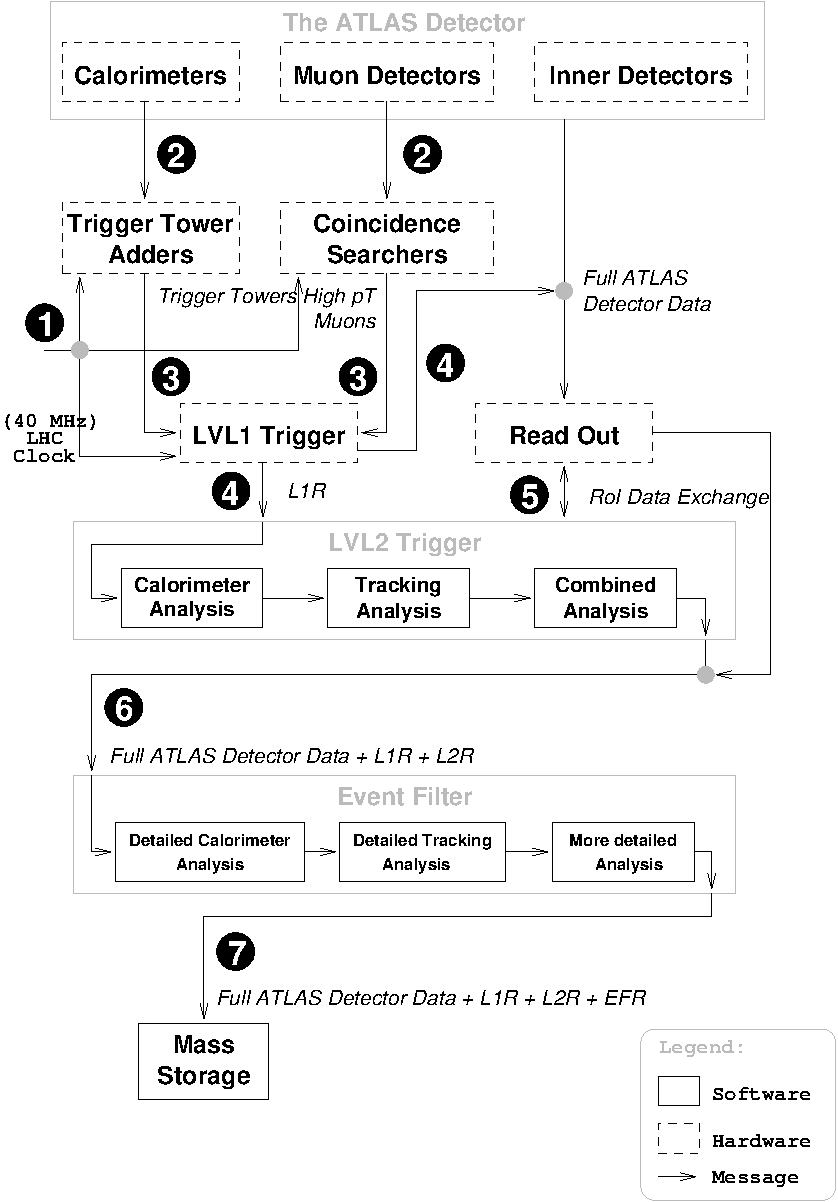
\includegraphics[scale=0.9]{trigger-physics}
\end{center}
\caption{Diagrama esquemático do Sistema de Filtragem do Experimento ATLAS
segundo suas funções de filtragem.}
\label{fig:trigger-physics}
\end{figure}

O processamento começa à medida que o LVL1 recebe o sinal do LHC acusando o
iminente cruzamento de pacotes (do inglês \eng{Bunch Crossing}) no ponto de
impacto (mensagem \ding{182}). Uma janela de aquisição de alguns nanossegundos
fará com que o Sistema de Leitura do LVL1 registre o evento (mensagem
\ding{183}). Os sistemas de pré-processamento são ativados em seguida.

No caso dos Calorímetros, somadores rápidos \cite{seixas:adder} agrupam as
informações das células dos calorímetros e.m. e hadrônicos, formando, para
cada seção, uma matriz de dados com granularidade reduzida
\cite{l1-tdr}. Estas macro-células ou ``torres'' de filtragem (do inglês,
\eng{Trigger Towers}, ou TT) agrupam os dados formando elementos com tamanho
igual a $0,1\times0,1$ no plano $\eta\times\phi$. Estes dois planos com
granularidade minimizada são varridos pelos diversos processadores do LVL1 e
os objetos de interesse, ou seja RoI's, localizados no detetor. Um processo
análogo é conduzido tendo por base os detetores de múons, com o objetivo de
encontrar objetos deste tipo (mensagem \ding{184}).

No final do processamento pelo LVL1, rapidamente depois da colisão, e no caso
de tratar de um evento interessante, uma mensagem contendo a localização dos
objetos encontrados por este nível de filtragem e variáveis indicando as
assinaturas pelo qual o evento foi aprovado, é repassada ao LVL2
(mensagem \ding{185}). Esta mensagem é chamada de Resultado do LVL1 (do inglês
\eng{LVL1 Result}) ou L1R, como visto na Seção~\ref{sec:lvl2arch}. Cabe-se
notar que o L1R pode conter múltiplas assinaturas em um único evento, no caso
deste conter elementos que confirmem mais de uma das linhas da
Tabela~\ref{tab:l1-rates}. Ademais, múltiplas RoI's secundárias podem estar
presentes na lista de objetos na mensagem. Em paralelo ao envio da mensagem em
direção ao LVL2, o LVL1 indica ao sistema de aquisição de dados (marcado na
figura como \eng{Read Out}) que carregue todos os dados do detetor em seus
\eng{buffers}.

O processamento no LVL2 é seqüencial. Ao receber um L1R, o Coordenador de
Execução do LVL2 (do inglês, \eng{Steering}) chamará um algoritmo de filtragem
para a confirmação do disparo do LVL1. O algoritmo em questão poderá
transferir, do sistema de leitura do detetor, a quantidade de dados que achar
necessária, ao redor da RoI, de forma a processá-la (mensagem \ding{186}). Se
não for possível rejeitar a assinatura do LVL1, o \eng{Steering} poderá chamar
mais e mais algoritmos até que o evento seja rejeitado ou definitivamente
aprovado ao Terceiro Nível de Filtragem ou Filtro de Eventos (do inglês
\eng{Event Filter} ou EF). Neste último caso, de forma equivalente à relação
entre o LVL1 e o LVL2, o LVL2 enviará um sumário indicando a razão da
aceitação do evento ao EF (mensagem \ding{187}). Este sumário contém valores
refinados de energia, momento e localização dos objetos explorados no contexto
LVL2. Analogamente ao resultado do LVL1, o resultado do LVL2 é chamado L2R (do
inglês {LVL2 Result}). Espera-se que o LVL2 atinja uma redução da taxa de
eventos de aproximadamente 25 vezes, de forma que o EF possa operar a uma taxa
de apenas alguns (1 ou 2)~kHz. O tempo médio de processamento para o LVL2 deve
estar na ordem dos 10~ms e para o EF, na ordem de alguns segundos, levando-se
em consideração o número de processadores disponíveis nestes níveis de
filtragem. No caso do evento ser aprovado pelo EF, é armazenado em mídia
permanente (mensagem
\ding{188}).

Os tempos de processamento-alvos representam a média de processamento por
evento. De fato, espera-se que eventos de interesse utilizem mais tempo de
processamento, enquanto que eventos pouco ou nada interessantes sejam
rapidamente descartados. Neste contexto, entende-se que, quanto menor o tempo
necessário e maior a qualidade da deteção dos diversos componentes do sistema
de filtragem, mais tempo computacional será despendido com a física de
interesse e menos recursos com eventos que representem física ordinária.

Diferetemente do LVL2, a análise no EF começa com 100\% dos dados do evento e
os resultados dos nível precedentes (L1R e L2R) já disponíveis na
memória. Neste nível de filtragem, correlações mais complexas podem ser feitas
entre as diferentes RoI's, e uma análise mais depurada do evento poderá ser
conduzida. Por exemplo, é possível fazer uso das RoI's secundárias para
atingir maior redução da taxa de eventos a ser registrada em mídia
permanente. Se aprovado, o evento é guardado, devidamente ``etiquetado'' e
repassado às fazendas de processamento \eng{offline} para posterior
reconstrução.

\section{Deteção de elétrons baseada em calorimetria}
\label{sec:e-detection}

O \eng{trigger} de elétrons ou fótons para o ATLAS conterá forte contaminação
de jatos com componentes hadrônicas (tipo descrito na Física Quântica
Cromo-dinâmica, do inglês Quantum Chromodynamics ou QCD), que formam o ruído
de fundo na deteção de elétrons \cite{nevski-calor-1992}. Estima-se que o
ruído de contaminação original esteja na ordem de $10^6$. O LVL1 do ATLAS poderá
excluir grande parte dos jatos QCD, se as conversões hadrônicas forem
importantes neste objeto, e apenas observando a quantidade de energia
hadrônica depositada na seção de mesmo nome dos calorímetros, mas terá pouca
eficiência em conversões com menos componentes hadrônicas. Estima-se em
\cite{daqnote00-02}, que a cada 25.000 objetos do tipo e.m., aprovados pelo
LVL1, apenas 1 será um elétron ou fóton verdadeiro. Somente no LVL2, o Sistema
de Filtragem, disporá do tempo e da completa granularidade do detetor para
executar uma seleção mais criteriosa, refinando a decisão obtida no LVL1
\cite{hlt-tdr} (mas originalmente discutida em \cite{ellis-calor-1992}). O
algoritmo de calorimetria também refina a posição do objeto originalmente
determinada pelo LVL1, de forma que algoritmos de deteção de traços,
reconhecidamente menos eficientes, possam reduzir sua área de procura. Por
estas razões, a correta identificação de elétrons é de suma importância para o
experimento.

A Figura~\ref{fig:e-shower} mostra a interação de um elétron com um detetor de
traços (\eng{Cloud Chambers}) e absorvedores de chumbo. Nesta figura, é
possível observar a formação de um chuveiro de partículas que diverge,
aproximadamente de forma isotrópica, do eixo de penetração do elétron. No caso
de elétrons \cite{wigmans-book}, a dispersão é menor que no caso de jatos de
partículas, já que há uma grande probabilidade de espalhamento múltiplo (do
inglês \eng{Multiple Scattering}) causado pelas componentes hadrônicas do
conjunto de partículas. A distância de penetração é diretamente proporcional à
energia do objeto em análise \cite{leo, knoll}, ainda que, para os mesmos
valores energéticos, jatos tendam a penetrar mais profundamente nos aparatos.

\begin{figure}
\begin{center}
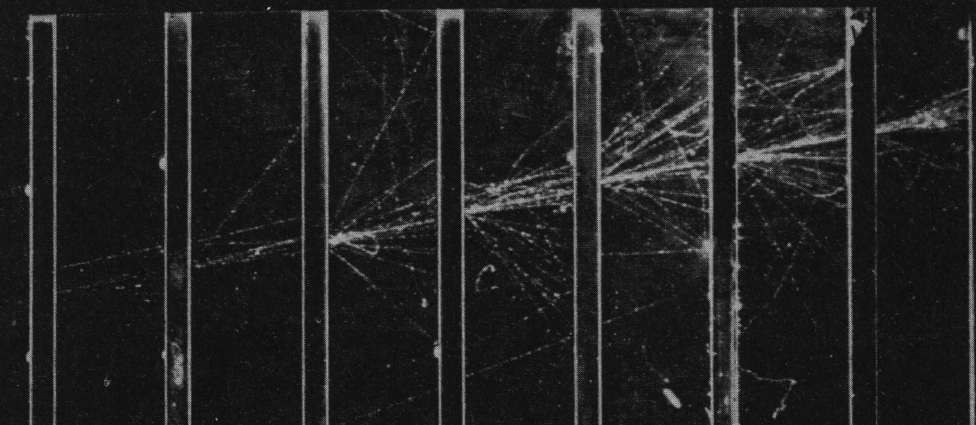
\includegraphics[scale=0.4]{e-cloud-chamber}
\end{center}
\caption{Interação de um elétron com um detetor de traços com absorvedores em
chumbo.} 
\label{fig:e-shower}
\end{figure}

%%CONSEGUIR FOTO DE UMA ROI COM O DÊNIS: ELECTRON, JET?

A deteção de elétrons beneficia-se deste conhecimento básico para
distingui-los de sua contaminação natural de jatos (e píons). Numa primeira
fase, chamada de Extração de Características, avalia-se, para uma região do
detetor, normalmente centralizada em um ponto pré-determinado, um conjunto de
valores que representem, o melhor possível, os perfis de deposição lateral (ou
radial) do objeto sendo estudado e sua penetração no aparato. Este processo
comprime\footnote{Para os fins deste trabalho define-se ``compressão'' ou
compactação a técnica pelo qual reduz-se a dimensionalidade de um sinal em um
espaço bem definido, preservando ou tentando preservar a informação relevante
que caracteriza este sinal de interesse. A transformação do espaço original
para o espaço ``comprimido'' é irreversível, salvo onde especificado.} a
informação de entrada, que normalmente possui dimensionalidade bastante
elevada (O(100)-O(1000)), para um conjunto pequeno (O(10)) de variáveis que
possam ser analisadas mais facilmente.

A questão da dimensionalidade da entrada está intimamente correlacionada com a
capacidade discriminatória do calorímetro. Quanto mais granular, maior
precisão pode ser obtida na definição de pontos de impacto e deteção de
partículas. O revés é o custo - detetores multi-segmentados são mais difíceis
e custosos de serem construídos.

No caso do experimento ATLAS (veja a Seção~\ref{sec:atlas-calo} para mais
detalhes), os calorímetros são segmentados em diversas camadas, e, camada a
camada, granularizados em células de deposição energética. A granularidade
varia camada a camada, pois cada uma delas possui um objetivo distinto de
emprego: as camadas iniciais têm por objetivo a discriminação de elétrons e
fótons e estimativa de posicionamento, as mais traseiras a deteção de
hádrons. As camadas da seção e.m. têm profundidade variante, sendo que a
segunda (EM2, a contar do zero, ou seja o pré-irradiador), tem a maior
profundidade de todas, ocupando mais de 80\% do volume total desta seção.

Para elétrons com valores energéticos até algumas dezenas de
gigaelétron-volts, espera-se que a maior parte da energia do objeto esteja
depositada nesta camada. A granularidade é bastante regular, tanto ao longo do
eixo $\eta$ quanto ao longo de $\phi$, como é possível observar na
Tabela~\ref{tab:lar}. Esta tabela também mostra o fator de compressão (ou
tamanho da torre de filtragem) $N_{\eta} \times N_{\phi}$ aplicado ao processo
de agrupamento necessário ao pré-processamento antes da análise feita pelo
LVL1.

A seção hadrônica dos calorímetro é bastante menos granular. O tamanho padrão
da célula ($0,1\times0,1$ no espaço $\eta\times\phi$) foi otimizado para
detetar hádrons. Esta classe de partículas penetra mais profundamente na
matéria e desenvolve complexas cascatas ao longo da penetração, normalmente
pouco interessantes. Entretanto, devem estar contidas no espaço do detetor. O
agrupamento padrão (torre de filtragem) para o LVL1 é de $2\times2$ células.

A Figura~\ref{fig:e-jet-deposit} mostra histogramas da relação da deposição
energética na seção hadrônica e a energia total do objeto considerando-se uma
área $0,4\times0,4$ no plano $\eta\times\phi$. Os eventos considerados são
simulações de elétrons e jatos cobrindo um campo energético de algumas dezenas
de GeV até 90 GeV interagindo com os calorímetros do ATLAS. Os eventos
selecionados passaram uma simulação realística do LVL1 e portanto representam,
todos, eventos que seriam classificados como elétrons por este nível de
filtragem. Observa-se que para jatos há uma probabilidade maior de depósito na
seção hadrônica que na seção e.m..

\begin{figure}
\begin{center}
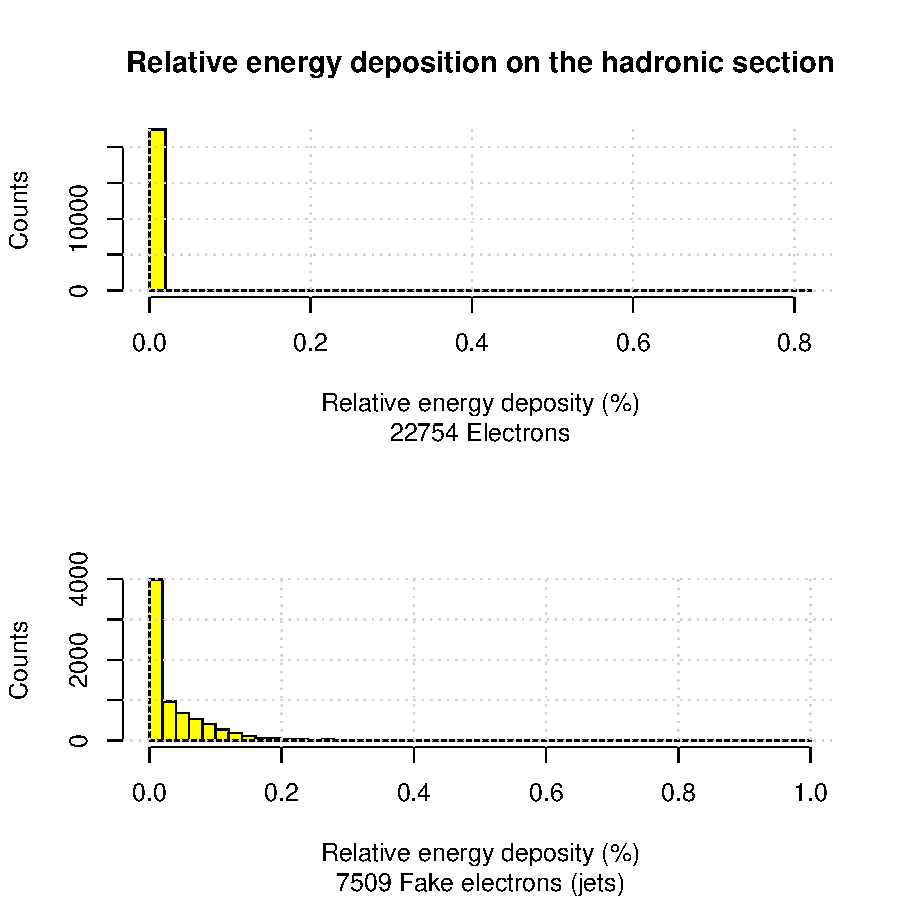
\includegraphics[scale=0.95]{em-had-percent}
\end{center}
\caption{Exemplo da relação de deposição energética na seção hadrônica e
energia total para elétrons (topo) e jatos (baixo).}
\label{fig:e-jet-deposit}
\end{figure}

Em seguida, aplica-se a discriminação da física de interesse. Tipicamente
\cite{nevski-calor-1992, guida-calor-1992, palutan-calor-2000}, a deteção é
realizada por meio da definição de patamares de separação (também ditos
\emph{cortes}) com informação \emph{a priori}. Este trabalho é normalmente
realizado por um físico experiente, de acordo com os canais físicos de maior
interesse para o experimento.

%É importante salientar que o melhor classificador baseado em cortes com
%informação \emph{a priori} também pode ser atingido iterativamente através de
%utilização de discriminadores lineares \cite{haykin-adaptative}, opcionalmente
%com atribuição de pesos para cada classe de partículas, definindo importâncias
%diferentes aos diferentes tipos de objetos estudados.

\section{Deteção de elétrons no LVL2}
\label{sec:lvl2-detect-electron}

O LVL1 (Seção~\ref{sec:lvl1}) executa seu procedimento de filtragem procurando
elementos nos calorímetros e detetores de múons que obedeçam a certos
critérios de classificação. A Tabela~\ref{tab:l1-rates}, mostrada
anteriormente, indica os principais objetos de interesse. No caso de objetos
e.m. (elétrons e fótons), o algoritmo pode ser resumido da seguinte forma:

\begin{enumerate}
\item Os sinais analógicos provenientes das células do detetor são agrupados
em macro-células chamadas Torres de Filtragem (do inglês \eng{Trigger Towers},
TT). A taxa de agrupamento não é uniforme, mas, em geral, forma TT's com
$0,1\times0,1$ no plano $\eta\times\phi$ para a seção eletromagnética do
calorímetro e $0,1\times0,1$ na seção hadrônica;

\item Os sinais somados das TT's são disponibilizados para a
lógica de leitura do LVL1;

\item Processadores especializados (4 no total) cobrem diferentes áreas do
detetor e utilizam um algoritmo de agrupamento, baseado em uma janela
deslizante \cite{l1-tdr} cobrindo uma região de $4\times4$ TT's (16 no
total), aqui resumido:

\begin{enumerate}
\item Se o núcleo de $2\times2$ TT's contiver energia maior que a
periferia, para um determinado patamar programável, um candidato a RoI é
definido;

\item Em seguida, somam-se, duas a duas, as energias transversas das TT's do
núcleo de $2\times2$ TT's e utiliza-se a maior das somas em uma comparação com
um patamar de energia EM;

\item Caso passe este critério, a energia na periferia da RoI-candidata é
verificada para assegurar o isolamento do objeto; 

\item O último critério é o isolamento hadrônico, onde o LVL1 verifica se não
há grande depósito de energia (transversa) na seção hadrônica.
\end{enumerate}  

No caso de atender a todos os pré-requisitos, o objeto candidato é promovido a
uma RoI tipo e.m.. Este algoritmo está representado na
Figura~\ref{fig:l1-calo}.
\end{enumerate}

\begin{figure}
\begin{center}
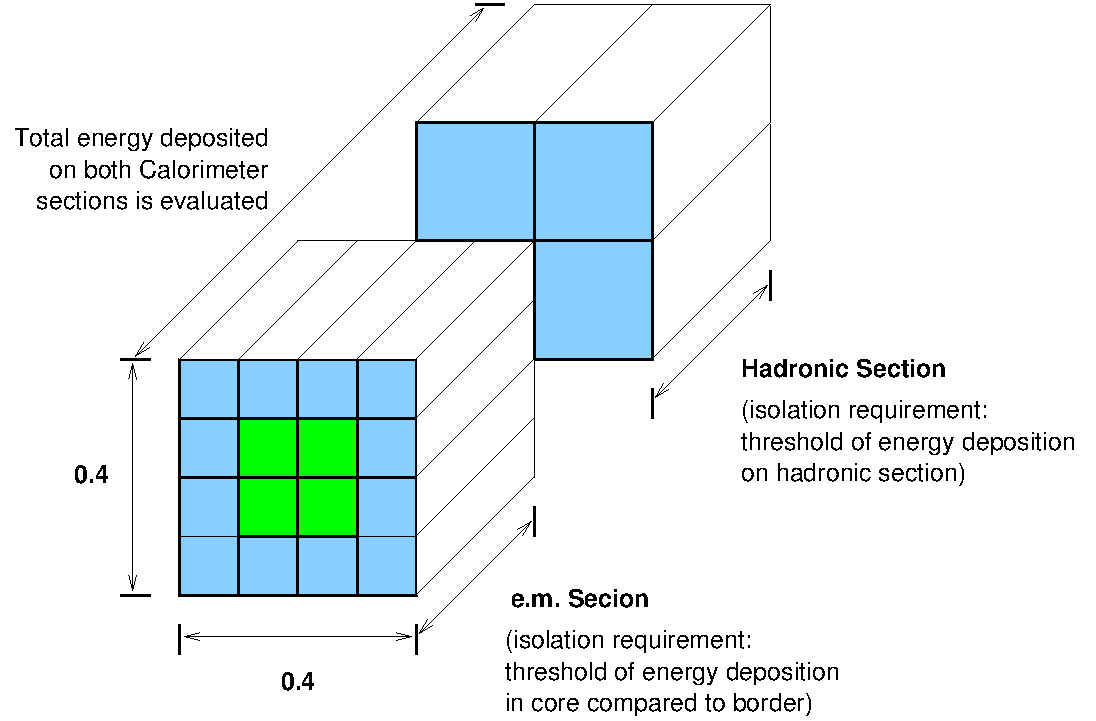
\includegraphics[scale=0.78]{l1-calo}
\end{center}
\caption{Representação gráfica do algoritmo de deteção de objetos e.m. no LVL1.}
\label{fig:l1-calo}
\end{figure}

Os diversos sub-módulos do LVL1 irão detetar e pré-classificar os elementos de
interesse para jatos, múons e energia faltante. Em seguida:

\begin{enumerate}
\item Os objetos detetados e seus pontos \textbf{centrais} de impacto
estimados no plano $\eta\times\phi$, ou seja, as RoIs, são encaminhados ao
Processador Central do Sistema de Filtragem do LVL1 (do inglês \eng{Central
Trigger Processor}, CTP) e uma decisão é feita levando-se em consideração as
assinaturas de interesse e resultados dos processamentos de outros módulos
(jatos, energia faltante e múons). A decisão de aprovar um evento é tomada
baseando-se em RoI's de acordo com critérios de preferência estipulados \eng{a
priori}. As RoI's que são utilizadas para a decisão de aprovação são rotuladas
``primárias'' ao passo que as demais, ``secundárias'';

\item Um sumário do resultado e das RoI's encontradas, já rotuladas (primárias
e secundárias) é repassado, através do \eng{RoI Builder} ao LVL2.
\end{enumerate}

O Segundo Nível de Filtragem do experimento ATLAS é a primeira vez onde o
evento será analisado tendo por base a granularidade máxima do detetor. O
objetivo deste nível de filtragem, de uma forma geral, é a confirmação das
informações do LVL1 e eventual depuração e extensão. Aproveitando-se de toda
a granularidade disponibilizada pelo sistema de leitura do detetor, o LVL2
começa analisando o evento através das RoI's classificadas como primárias pelo
LVL1.

Ao receber as informações das RoI's o \eng{Steering} ativará o passo de
decodificação do resultado do LVL1 e, em seguida, selecionará a próxima fase
de análise, que dependerá diretamente do tipo RoI's primárias do evento. No
caso de RoI's do tipo e.m., um algoritmo de deteção de elétrons (e fótons)
será ativado.

\section{Deteção de elétrons no LVL2 do ATLAS}
\label{sec:classic-detection}

Como discutido anteriormente, na Seção~\ref{sec:e-detection}, o processo de
deteção veloz baseado em calorimetria pode ser sub-dividido nas seguintes partes:

\begin{enumerate}
\item Compactação do sinal de entrada;
\item Deteção da física de interesse baseada no espaço comprimido.
\end{enumerate}

Para o ATLAS, a fase de compactação irá mapear o espaço de entrada definido
pelas células da RoI send tratada em 4 variáveis com alto poder
discriminatório, baseado na percepção da física de interesse e da contaminação
esperada. No caso de elétrons, espera-se que haja forte contaminação de jatos
com muitas componentes e.m.. Desta forma, a compactação da informação de entrada
tentará realçar informações como a dispersão do objeto na RoI ou a
profundidade de interação do objeto com as diversas camadas do detetor.

O nome do algoritmo usado para a FEx de RoI's primárias tipo e.m. é
\emph{T2Calo}, uma variação das palavras \eng{Trigger}, LVL2 e
Calorimetria. As variáveis extraídas do \eng{cluster} definido pela RoI do
LVL1, por este algoritmo, estão descritas a seguir. Cada uma destas variáveis
define uma etapa ou mais etapas do processamento do T2Calo que está
esquematizada nas figuras correspondentes:

\begin{enumerate}
\item \textbf{Energia do núcleo e.m.}, Figura~\ref{fig:t2calo-1}: O
primeiro passo do algoritmo é um refinamento do centro da RoI. Isto é feito
encontrando-se o pico de deposi\-ção ener\-gé\-tica na segunda camada da
se\-ção eletroma\-gné\-tica do calo\-rí\-metro, que é tam\-bém a mais profunda
desta se\-ção (veja uma discus\-são mais detalhada da geometria do detetor na
Seção~\ref{sec:atlas-calo}). O valor do centro da cé\-lula é tomado como uma
nova estimativa de posicionamento da RoI e será utilizado para os cál\-culos
seguintes.

Em seguida, ainda utilizando-se dos dados da segunda camada e.m., calcula-se a
soma dos valores de deposição energética numa região de tamanho
$\Delta_\eta=0,075\times\Delta_\phi=0,175$ e numa região de tamanho
$\Delta_\eta=0,075\times\Delta_\phi=0,175$, ao redor do centro de impacto
encontrado anteriormente. De posse destes valores, a primeira característica
será extraída:

\begin{equation}
\rcore \text{ ou } R_\text{core} = \frac{\text{Energia}^{e.m.2}_{\Delta_\eta=0,075\times\Delta_\phi=0,175}}{\text{Energia}^{e.m.2}_{\Delta_\eta=0,175\times\Delta_\phi=0,175}}
\end{equation}

Esta quantidade tenta estimar o espalhamento da cascata formada pelo
decaimento do objeto na RoI. No caso do objeto ser um jato, espera-se que a
cascata tenha um espalhamento maior que no caso de elétrons, resultando em um
valor menor que 1 para esta quantidade;

\begin{figure}
\begin{center}
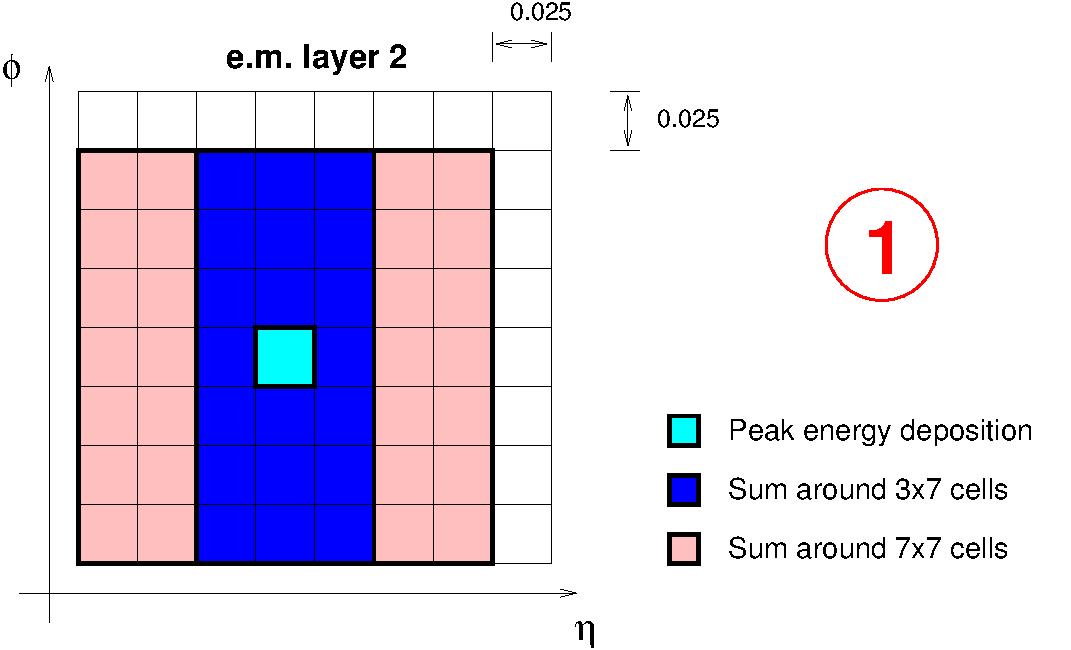
\includegraphics[scale=0.725]{t2calo-1}
\end{center}
\caption{T2Calo, Etapa 1: Cálculo do centro refinado e deposições de
energia na segunda camada e.m., para regiões de tamanho
$\Delta_\eta=0,075\times\Delta_\phi=0,175$ e
$\Delta_\eta=0,175\times\Delta_\phi=0,175$.} 
\label{fig:t2calo-1}
\end{figure}

\item \textbf{Máximos na primeira camada e.m.}, Figura~\ref{fig:t2calo-2}: Os
dois maiores picos de energia na primeira camada da seção e.m. (denominados
$E_1$ e $E_2$ respectivamente) são detetados. De posse destes valores, a
segunda característica é extraída:

\begin{equation}
\eratio \text{ ou } E_\text{ratio} = \frac{E_1-E_2}{E_1+E_2}
\end{equation}

Uma vez que jatos de par\-tí\-culas interagem de forma mais espalhada do que
e\-lé\-trons, espera-se que, na primeira camada e.m., sejam observados vários
picos. Desta forma, se o objeto for um elétron (objeto único), espera-se que
$E_2=0$, já que a cascata de partículas que o elétron forma na sua interação
com o calorímetro é, tipicamente, bastante estreita. Assim sendo, para
elétrons, \eratio tenderá a 1. Para jatos, normalmente, \eratio\ será menor
que 1, já que $E_2 \neq 0$.

\begin{figure}
\begin{center}
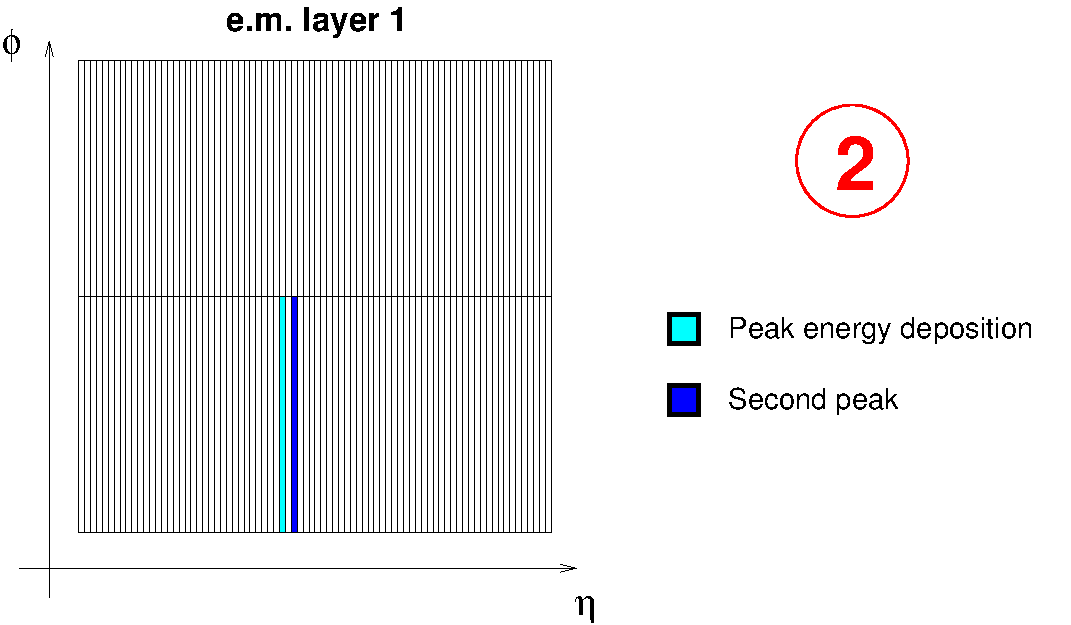
\includegraphics[scale=0.8]{t2calo-2}
\end{center}
\caption{T2Calo, Etapa 2: Procura dos dois maiores picos na primeira camada e.m..}
\label{fig:t2calo-2}
\end{figure}

\item \textbf{Energia e.m.}, Figura~\ref{fig:t2calo-3}: Os valores parciais de
deposição energética para cada camada da seção e.m., numa região de
$\Delta_\eta=0,075\times\Delta_\phi=0,175$ ao redor do pico de deposição
energética na segunda camada, também são calculados. Destas somas parciais, a
terceira característica da RoI é calculada somando-se estes 4 valores. O valor
original calculado é dividido pelo $\cosh{|\eta|}$ para que obtenha-se a
energia transversa\footnote{O termo ``transverso'' neste contexto refere-se ao
feixe de partículas.} (projetada no plano $x \times y$ do detetor). Espera-se
que a energia de elétrons esteja totalmente contida nesta janela; por sua vez,
jatos devem apresentar uma fração menor de sua energia depositada nesta área;

\begin{figure}
\begin{center}
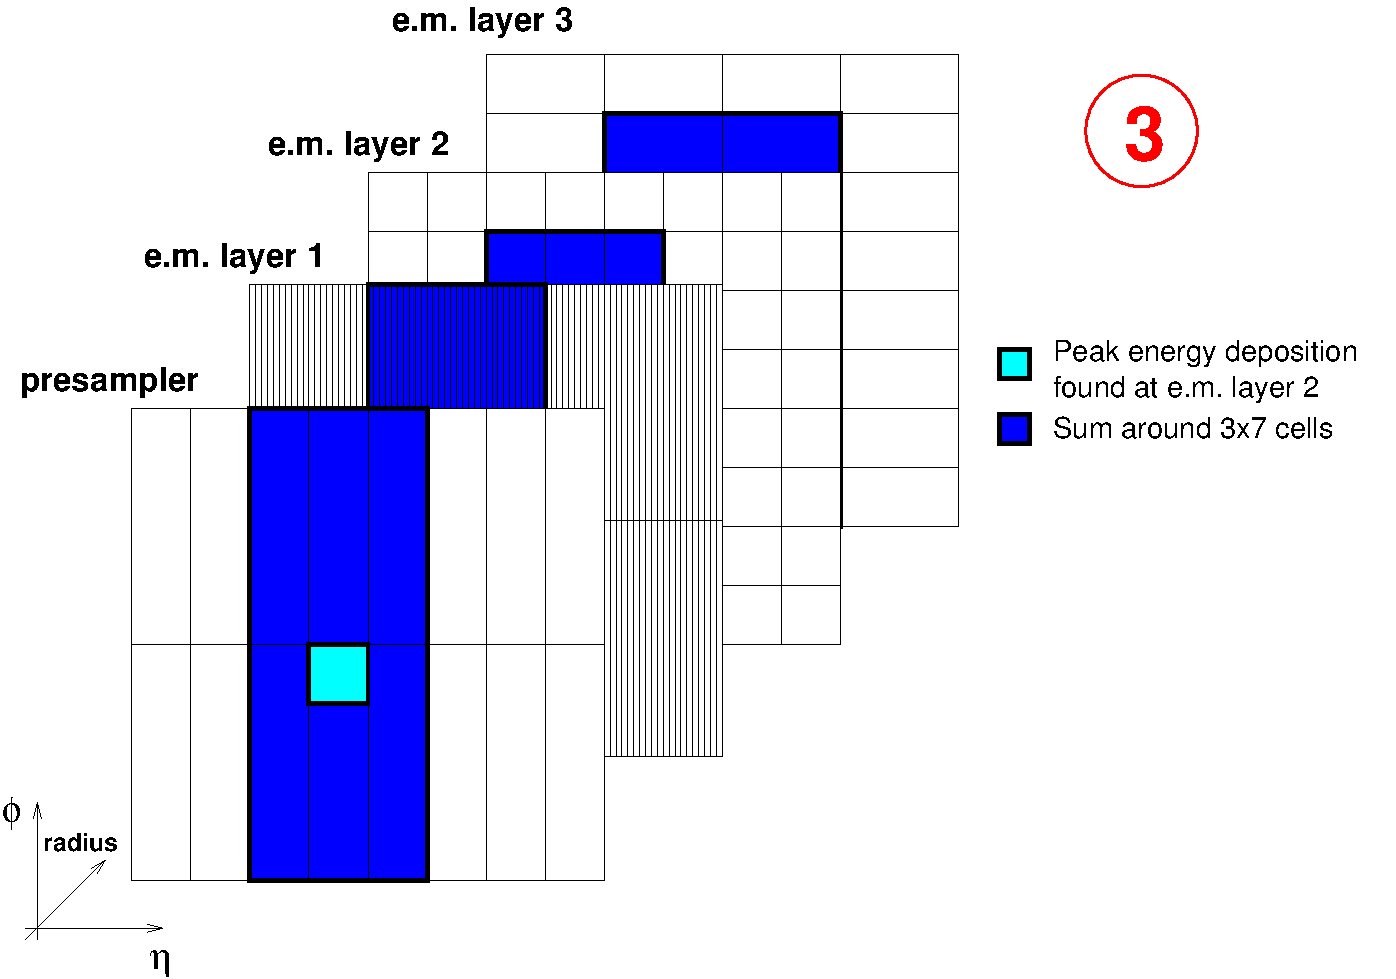
\includegraphics[scale=0.55]{t2calo-3}
\end{center}
\caption{T2Calo, Etapa 3: Cálculo dos somatórios parciais de energia por
camada, em uma área equivalente a $\Delta_\eta=0,075\times\Delta_\phi=0,175$.}
\label{fig:t2calo-3}
\end{figure}

\item \textbf{$\text{Energia
Hadrônica}_{\Delta_\eta=0,2\times\Delta_\phi=0,2}$}: Calcula-se a energia
total numa região $\Delta_\eta=0,2\times\Delta_\phi=0,2$, centrado no pico de
deposição energética na segunda camada e.m.. Este procedimento é executado
para cada camada na seção hadrônica, e depois uma somatório do total
transverso é executado. Para elétrons, a quantidade de energia depositada na
camada hadrônica deve ser próxima de zero, enquanto que, para jatos, espera-se
que seja diferente de zero.

\begin{figure}
\begin{center}
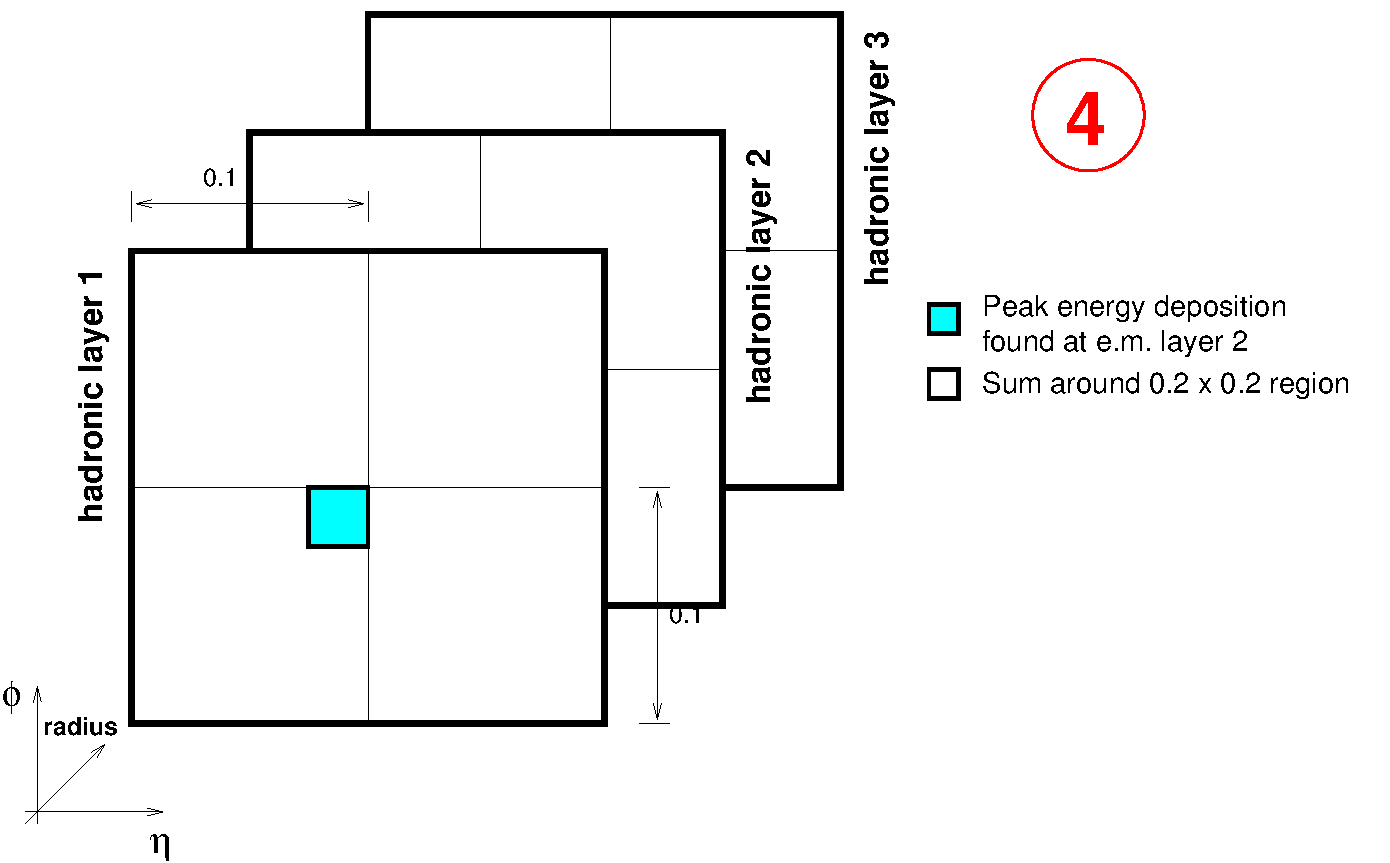
\includegraphics[scale=0.6]{t2calo-4}
\end{center}
\caption{T2Calo, Etapa 4: Valores parciais e somatório das energias, em uma
área equivalente a $0,2\times0,2$ no plano $\eta\times\phi$, para as camadas
da seção hadrônica.} 
\label{fig:t2calo-4}
\end{figure}

\end{enumerate}

O algoritmo de deteção propriamente dito segue a execução do T2Calo e é
chamado \emph{EGammaHypo}. Este algoritmo tem a função exclusiva de combinar
as informações disponibilizadas à partir do processo de extração de
características e tomar uma decisão simples baseada nas propriedades físicas
das partículas de interesse. A seqüência discriminatória empregada pelo
EGammaHypo está representada a seguir, em pseudo-código: 

\newcommand{\textbu}[1]{\textbf{\underline{#1}}}
\newcommand{\IF}[1]{\textbu{se} #1, \textbu{então}}
\newcommand{\RETURN}[1]{\\ \textbu{retornar} #1\textbf{;}}
\newcommand{\lumihi}{\ensuremath{10^{33} \text{cm}^{-2}\text{s}^{-1}}}

\begin{description}
\item[\ding{182}] \IF{$\rcore \lessapprox \text{corte}_{\rcore}$}
	\RETURN{\textbf{não é} elétron}

\item[\ding{183}] \IF{$\eratio \lessapprox \text{corte}_{\eratio}$}
	\RETURN{\textbf{não é} elétron}

\item[\ding{184}] \IF{$\etem \lessapprox \text{corte}_{\etem}$}
	\RETURN{\textbf{não é} elétron}

\item[\ding{185}] \IF{$\ethad \gtrapprox \text{corte}_{\ethad}$}
	\RETURN{\textbf{não é} elétron}

\end{description}

Se o objeto definido pelo LVL1 conseguir passar todos os critérios definidos
neste procedimento, é promovido a ``candidato à elétron'' dentro do LVL2. As
fases seguintes de discriminação tentarão encontrar um traço, com momento
equivalente a energia do \eng{cluster}, e uma nova rodada de hipóteses
confirmará (ou não) o possível elétron. A procura de traços nos detetores
internos é um procedimento tipicamente lento (na ordem de dezenas, dependendo
centenas de milissegundos \cite{hlt-tdr}), e deve ser evitada tanto quanto
possível. Por outro lado, deseja-se que o sistema de deteção preliminar,
baseado em calorimetria, seja o mais rápido possível, e mantenha bons níveis
de discriminação, como já discutido.

Uma das estratégias em consideração atualmente, pondera sobre a utilização dos
diversos estágios de hipótese de forma seqüencial, durante a extração de
característica. Neste caso, após interagir com a segunda camada e.m., o T2Calo
seria brevemente suspenso e a primeira das hipóteses verificada, criando
recursos para uma rejeição mais antecipada. Em seguida, os dados da RoI para a
primeira camada e.m. seriam carregados no processador, a segunda variável
seria calculada e mais uma rodada de decisão seria tomada. As próximas etapas
seriam a carga dos dados da terceira camada e.m. e do pré-irradiador,
seguindo-se da análise de dados na seção hadrônica.

\subsection{Ajuste fino para cada canal}

Para cada uma das assinaturas de interesse aprovadas pelo LVL1, o segundo
nível contará com algoritmos e sistemas de hipótese adequados àquela física. É
interessante notar que, mesmo para os canais similares, e.g. (veja a
Tabela~\ref{tab:l1-rates}) \texttt{EM25i} e \texttt{EM15i}, os cortes impostos
pelo algoritmo de hipótese serão otimizados para estas categorias de energia.

%Neste trabalho estaremos comparando os diversos algoritmos de deteção
%utilizando um conjunto de eventos destinado ao estudo da discriminação
%elétron/jato no contexto da assinatura mais freqüente do experimento:
%\texttt{EM25i}.

\section{Caracterização do T2Calo e do EGammaHypo}
\label{sec:def-eghypo}

Para a caracterização de operação do T2Calo e do algoritmo de hipótese
associado, o EGammaHypo, os seguintes grupamentos de dados foram
considerados:

\begin{itemize}
\item Cerca de 23.000 elétrons simulados via Monte Carlo, proveniente de
interações tipo $H (130 \text{GeV})\rightarrow ZZ \rightarrow 4e^-$ e 
$H (130 \text{GeV})\rightarrow ZZ \rightarrow 2e^- + 2\mu$. Os elétrons de
cada evento simulado interagem com diferentes regiões do detetor;
\item Cerca de 250.000 jatos-duplos, simulados via Monte Carlo, com energia total,
fixa em 25 GeV, também interagindo com várias partes do detetor.
\end{itemize}

Nos dois casos, considerou-se simulações com ruído, proveniente da eletrônica,
e uma planta de detetor compatível com o que está sendo instalado atualmente
na caverna do experimento, provendo um ambiente bastante acurado dentro do que
é possível prever-se em termos de operação, mas ainda exeqüível para um
ambiente de simulação.

Esta massa original de dados foi submetida a uma simulação do LVL1, que
implementa o algoritmo discutido na Seção~\ref{sec:lvl2-detect-electron},
aceitando todos os eventos com objetos tipo EM com as seguintes
características:

\begin{itemize}
\item ao menos 10 GeV numa região de $2\times2$ torres de filtragem na seção
e.m.;
\item no máximo 4 GeV na região periférica ao núcleo de $2\times2$ torres de
filtragem; 
\item no máximo 2 GeV de depósito na seção hadrônica;
\item qualquer valor para o centro em $\phi$;
\item $\eta$ variando de $-2,5$ a $+2,5$;
\end{itemize}

Um total de cerca de 22.000 elétrons e 7.000 fazem parte da massa de dados
remanescente após a aplicação dos cortes acima. A
Figura~\ref{fig:transverse-energy} contém os histogramas de deposição
energética total transversa de elétrons e jatos, em uma janela de $0,4 \times
0,4$ no plano $\eta\times\phi$, considerando-se as duas seções do calorímetro
(e.m. e hadrônica). É possível distinguir um corte acentuado nas redondezas de
aproximadamente 10~GeV, que equivale à ação da simulação do LVL1, como
esperado. Para o histograma de jatos a média aproxima-se ao valor esperado de
25~GeV, exibindo um pico pronunciado ao redor deste valor. Como observa-se,
grande parte dos jatos encontram-se com valor de energia transversa entre 10 e
40~GeV, enquanto que para elétrons, a distribuição decai suavemente até
$\approx$ 91~GeV (aproximadamente a massa de repouso do bóson Z).
%Antes do corte, é possível distinguir uma cauda, se estendendo até a
%origem. Este fenômeno pode ser observado no LVL2 já que os valores de
%calibração de energia aplicados às células do calorímetro neste nível de
%filtragem não estão disponíveis ao nível de filtragem anterior.

% Interessante observar que isto poderá e deverá influenciar nos resultados
% disponíveis, mas o que deseja-se demonstrar é a técnica e não uma solução
% pronta para o problema.

\begin{figure}
\begin{center}
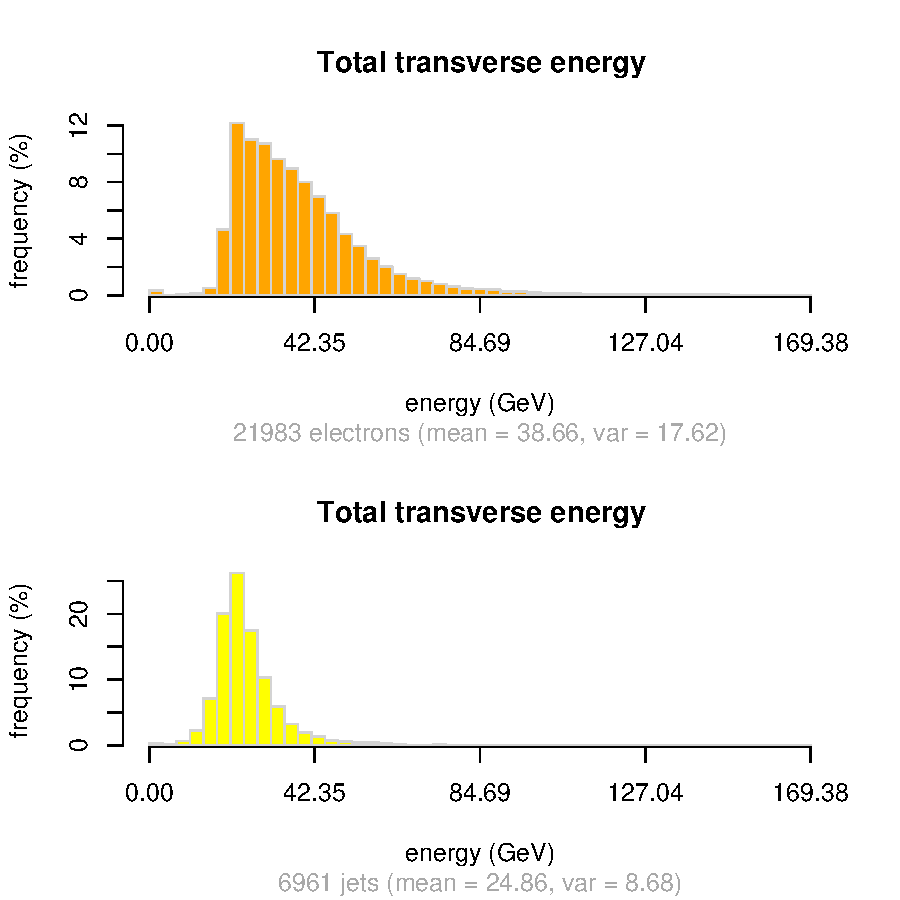
\includegraphics[scale=0.95]{transverse-energy}
\end{center}
\caption{A deposição total de energia em uma região $0,4 \times 0,4$ no plano
$\eta\times\phi$ para elétrons (em cima) e jatos (em baixo) para a massa de
dados disponível para o estudo.}
\label{fig:transverse-energy}
\end{figure}

As Figuras~\ref{fig:em-tenergy} e \ref{fig:had-tenergy} mostram histogramas da
energia transversa total por seção de calorimetria para e\-lé\-trons e
jatos. Nota-se que, para elétrons, quase 100\% da energia total do objeto é
retida na seção e.m., enquanto que, para jatos, observa-se algum vazamento de
energia na seção hadrônica. Embora o corte realizado pelo LVL1 tenha sido em
2~GeV para o vazamento de energia nesta seção, observa-se uma quantidade não
desprezível de eventos com energia hadrônica além deste valor. Por outro lado,
a energia total neste seção decai rapidamente e assume-se que a existência
desta cauda esteja relacionada a (baixa) qualidade da calibração dos dados
utilizada no LVL1.

\begin{figure}
\begin{center}
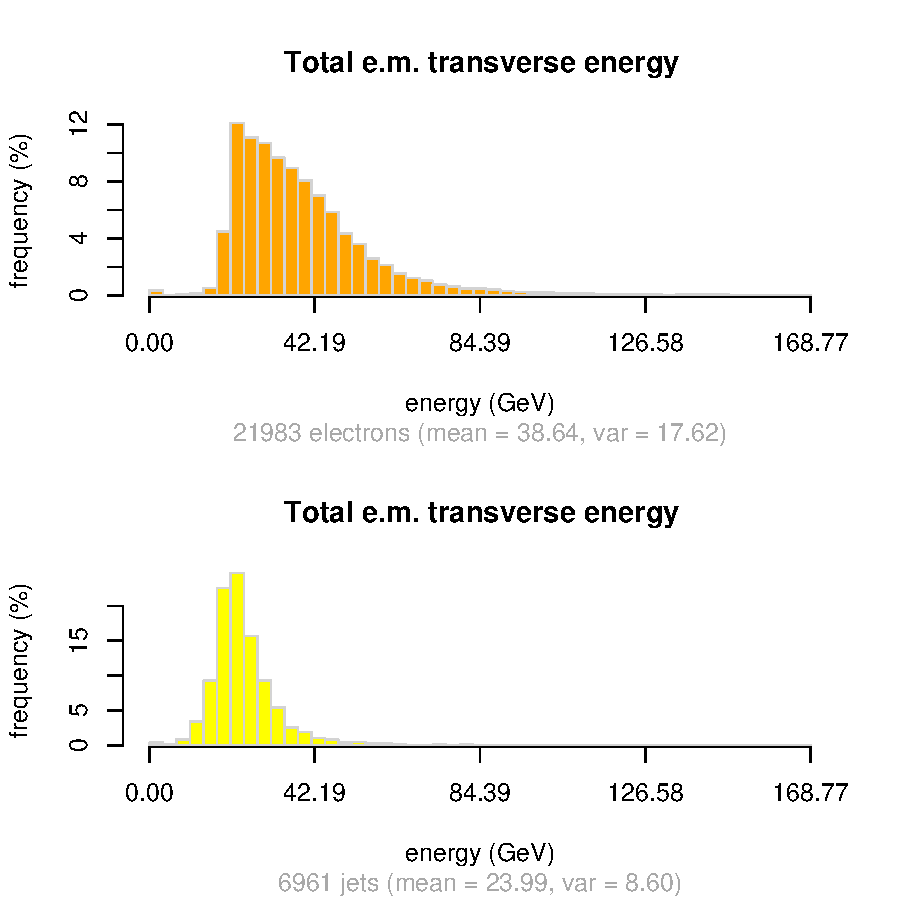
\includegraphics[scale=0.95]{em-tenergy}
\end{center}
\caption{A deposição total de energia na seção e.m. em uma região $0,4 \times
0,4$ no plano $\eta\times\phi$ para elétrons (em cima) e jatos (em baixo) para
a massa de dados disponível para o estudo. As contagens estão normalizadas.}
\label{fig:em-tenergy}
\end{figure}

\begin{figure}
\begin{center}
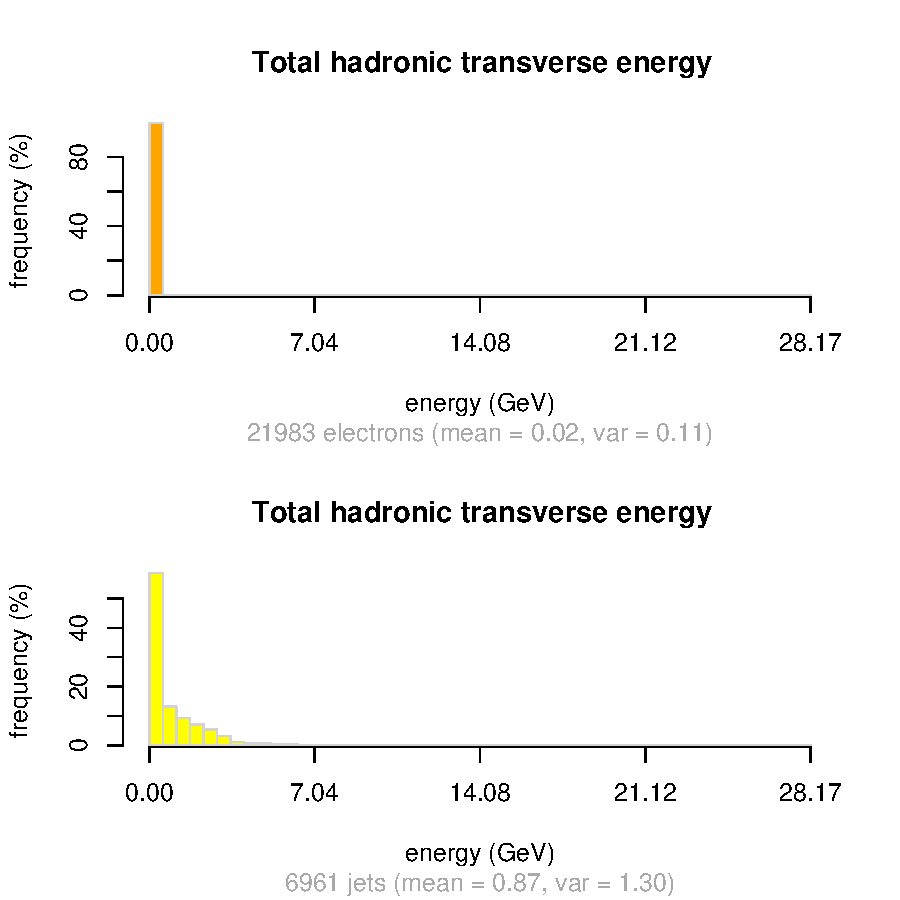
\includegraphics[scale=0.95]{had-tenergy}
\end{center}
\caption{A deposição total de energia na seção hadrônica em uma região $0,4 \times
0,4$ no plano $\eta\times\phi$ para elétrons (em cima) e jatos (em baixo) para
a massa de dados disponível para o estudo. As contagens estão normalizadas.}
\label{fig:had-tenergy}
\end{figure}

As Figuras~\ref{fig:rcore} e \ref{fig:eratio} mostram, respectivamente, a
fração \rcore e \eratio, tal como utilizada pelo EGammaHypo para definir a
eficiência de deteção de elétrons e jatos. Na Figura~\ref{fig:rcore},
observa-se que a distribuição para elétrons tem média bastante próxima a 1 e
baixíssima variância. Para jatos, a média é mais baixa e a distribuição
apresenta longa cauda em direção à origem. No caso da variável \eratio, que
tem por objetivo detetar picos de deposição energética na primeira camada
e.m., para elétrons observa-se um pico dominante em 1, ao passo que, para
jatos, há uma distribuição mais uniforme, indicando uma separabilidade
linear.

\begin{figure}
\begin{center}
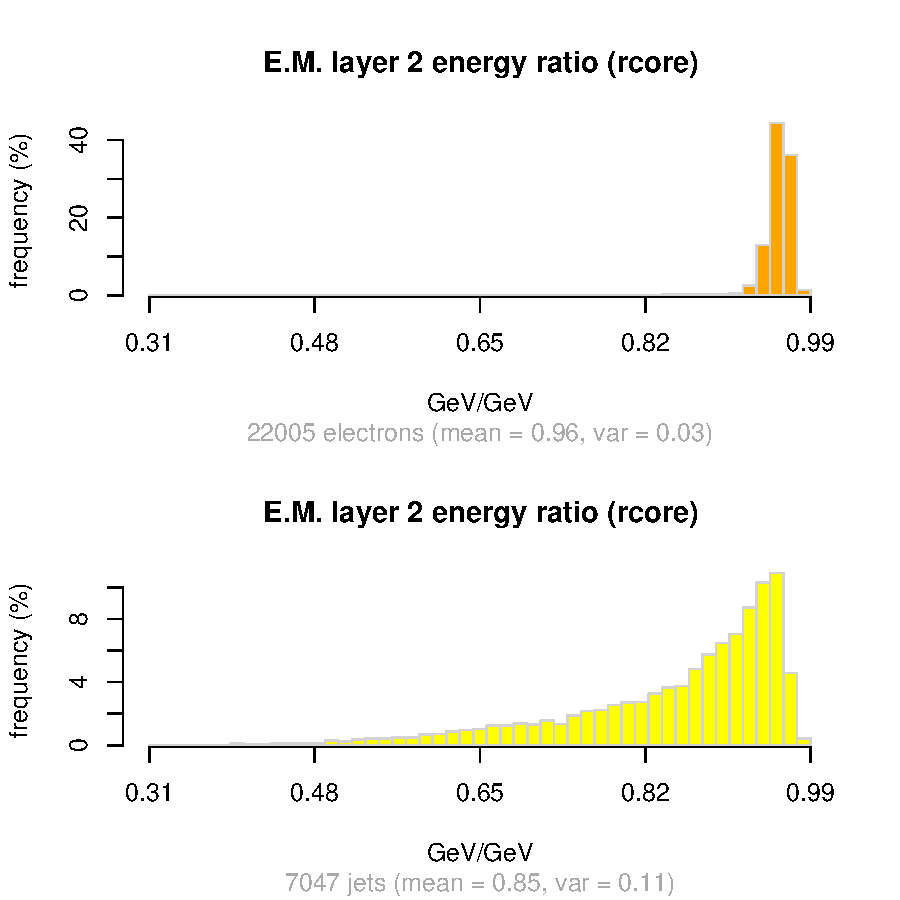
\includegraphics[scale=0.95]{rcore}
\end{center}
\caption{Distribuição da variável \rcore para elétrons (em cima) e jatos
(embaixo). As contagens estão normalizadas.}
\label{fig:rcore}
\end{figure}

\begin{figure}
\begin{center}
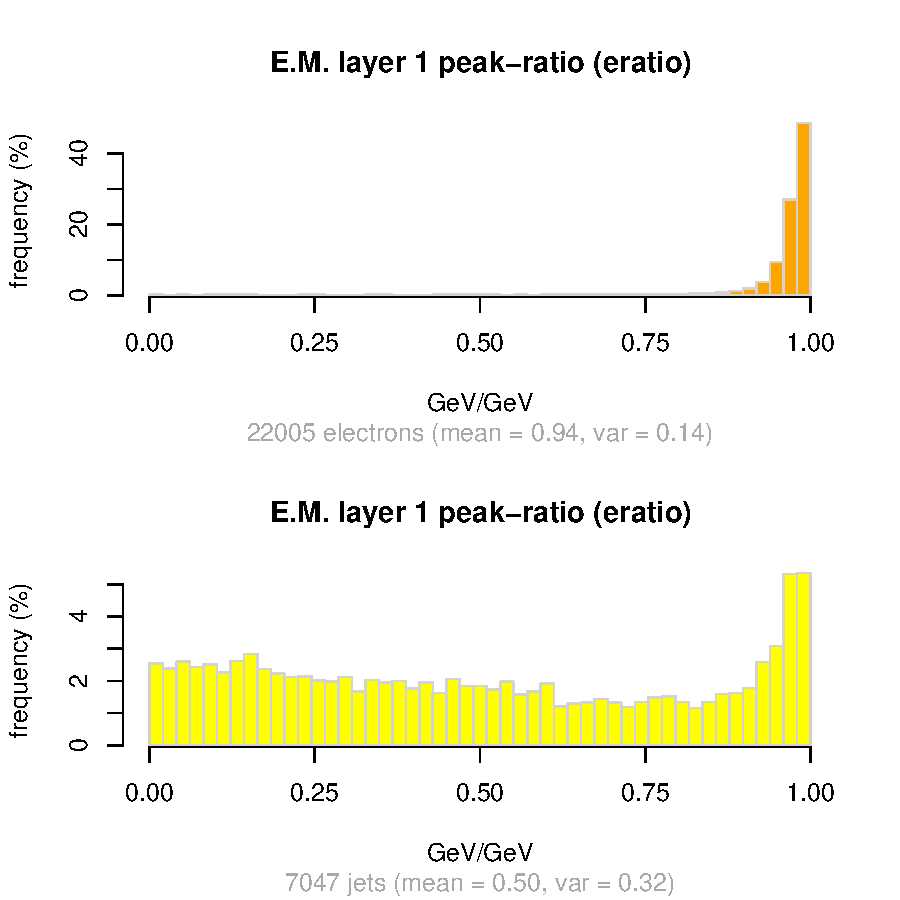
\includegraphics[scale=0.95]{eratio}
\end{center}
\caption{Distribuição da variável \eratio para elétrons (em cima) e jatos
(embaixo). As contagens estão normalizadas.}
\label{fig:eratio}
\end{figure}

As Figuras~\ref{fig:eta} e \ref{fig:phi} mostram histogramas para elétrons e
jatos dos centros refinados pelo T2Calo das RoI's em questão, tanto em relação
à variável $\eta$ quanto à variável $\phi$. É possível distinguir uma
uniformidade na distribuição em $\phi$ e uma tendência a concentração de
eventos nas proximidades de $\eta=0$, como é aguardado no experimento.

\begin{figure}
\begin{center}
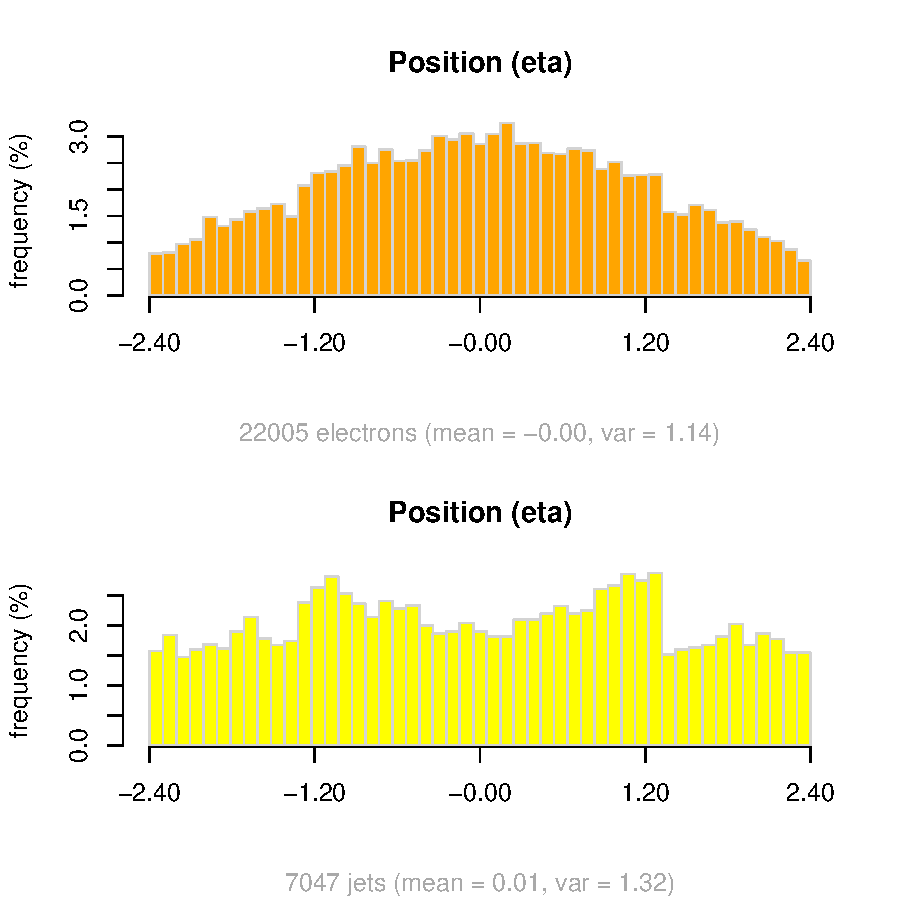
\includegraphics[scale=0.95]{eta}
\end{center}
\caption{Distribuição em $\eta$ dos centros refinados das RoI's para elétrons
(em cima) e jatos (embaixo). As contagens estão normalizadas.}
\label{fig:eta}
\end{figure}

\begin{figure}
\begin{center}
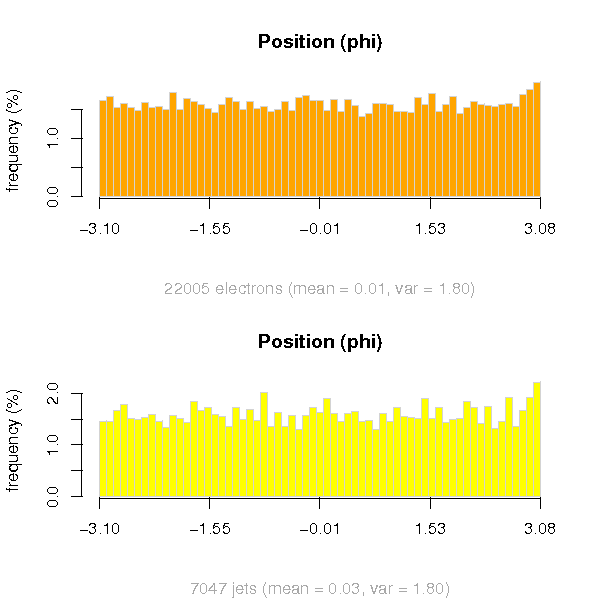
\includegraphics[scale=0.95]{phi}
\end{center}
\caption{Distribuição em $\phi$ dos centros refinados das RoI's para elétrons
(em cima) e jatos (embaixo). As contagens estão normalizadas.}
\label{fig:phi}
\end{figure}

Exceto por eventuais problemas na lógica de simulação (Monte Carlo) e
filtragem (pelo LVL1), estima-se que a massa de dados seja representativa do
problema da separação entre jatos e elétrons. Deve ser levado em consideração
que, para jatos, o pico ao redor de 25~GeV poderá introduzir imprecisões na
definição da capacidade de deteção de elétrons bastante energéticos, presentes
na massa de estudo. Sempre que possível, tentar-se-á levar estas restrições em
consideração.

\subsection{Deteção de elétrons com o EGammaHypo e sua otimização}
\label{sec:eghypo}

Para que a eficiência de deteção do algoritmo proposto pelo EGammaHypo seja
estimada, deve-se passar a massa de dados de estudo por um processo de
otimização que ajude o especialista a selecionar os patamares de corte que
definem o algoritmo, como exposto na Seção~\ref{sec:classic-detection}. Para
tal, dividiu-se o conjunto de dados em 2 metades com aproximadamente o mesmo
número de RoI's. A primeira metade será utilizada para o ``treinamento'' ou
otimização dos cortes, enquanto que a segunda será utilizada para o teste dos
cortes de forma que seja possível testar se, para uma massa de dados jamais
apresentada ao sistema, a eficiência de deteção está de acordo com aquele
encontrada durante a determinação dos cortes. Desta forma, saberemos se o
detetor está demasiado especializado nos dados presentes no conjunto de
treinamento ou pode ser utilizado \emph{genericamente} para a deteção de
elétrons e jatos.

O algoritmo de otimização não será exaustivo, varrendo todo o espaço de dados,
mas partirá de patamares pré-fixados em valores intuitivos e definirá uma
sub-área de variação por onde testará exaustivamente as combinações dos 4
cortes necessários, como é normalmente feito atualmente. Eis aqui os patamares
e passos de busca (ou \emph{possibilidades}) que utilizaremos:

\begin{enumerate}
\item Corte em \rcore: de 0,6 a 1,0, em passos de 0,01 (41 possibilidades);
\item Corte em \eratio: de 0,6 a 1,0, em passos de 0,01 (41 possibilidades);
\item Corte em \etem: de 5000 a 30000 MeV em passos de 500 MeV (51
possibilidades);
\item Corte em \ethad: de 0 a 4000 MeV em passos de 500 MeV (9
possibilidades). 
\end{enumerate}

Para cada corte, a totalidade da massa de dados de treinamento do método é
avaliada e as RoI's que \textit{sobrevivem} ao corte são levadas à próxima
etapa. As eficiências relativas e a quantidade de dados utilizadas para o teste
da fase seguinte são acumulados para posterior análise. Levando-se em
consideração o número combinações dadas as possibilidades do problema de
otimização e considerando-se que a superfície de erro não possua um único
mínimo, há de se tentar $41 \times 41 \times 51 \times 9 = 771579$ diferentes
combinações, neste caso, antes de qualquer conclusão.

Está claro que uma varredura completa do espaço de parâmetros,
i.e. buscando-se todo o espaço de possibilidades ao invés dos sub-conjunto
utilizados, estaria fora de questão para uma utilização em condições que
possam variar em questão de horas, como é o caso do experimento ATLAS. Desta
forma, seja uma antecipação para os cortes seria necessária ou uma redução do
espaço de busca permitindo uma otimização mais rápida. A utilização de
programas especialmente codificados para a tarefa também poderia diminuir o
tempo de teste, tornando o método mais atraente para uma utilização prática.

A Figura~\ref{fig:eghypo-best-sp-train} mostra os resultados da busca
exaustiva definida anteriormente. Esta figura de mérito, normalmente chamada
de \textit{Característica de Operação do Receptor} (do inglês,
\eng{Receiver Operating Characteristics}, ROC \cite{vantrees}), contém os
resultados de cada ponto de operação do algoritmo EGammaHypo. O eixo vertical
denota a eficiência na deteção do sinal de interesse (elétrons), enquanto o
eixo horizontal, a taxa de falso-alarme (erro em jatos) naquele ponto de
operação. A taxa de falso alarme é escalonada em 25~kHz, que é a taxa máxima
de ruído de fundo esperada. O valor do eixo horizontal portanto, denota a
quantidade de jatos que serão aprovados pelo LVL2, como elétrons e, portanto,
representa uma medida direta da taxa de eventos descarregados no Filtro de
Eventos.

Observa-se que, para o conjunto de intervalos testado, a massa de resultados
assume uma forma angulada. Ao redor do ponto de flexão, na parte exterior da
massa de resultados, encontraremos as melhores relações de eficiência
\textit{versus} falso-alarme para este discriminador. O ponto destacado nesta
figura representa o conjunto de cortes que maximiza a multiplicação da soma
eficiências de deteção pelo produto entre elas, ou seja:

\begin{equation}
SP = (\text{efic.}_{classe_1} + \text{efic.}_{classe_2}) \times
(\text{efic.}_{classe_1} \times \text{efic.}_{classe_2})
\label{eq:sp-product}
\end{equation}

O produto SP de um detetor para 2 classes de eventos apresenta um máximo
($=2,0$) quando a eficiência na deteção de ambas as classes é máximo
(i.e. $=1,0$), e um mínimo em $0$ quando a eficiência de deteção de
\textbf{qualquer} uma das duas classes de eventos é $0$. É interessante notar
que, para um determinado classificador, o valor do máximo da
Equação~\ref{eq:sp-product} indicará o ponto de inflexão da curva R.O.C.. Este
ponto determina a melhor relação de deteção entre as duas classes de eventos
para o classificador.

À medida que a curva R.O.C. se aproxima, em detrimento de uma melhora na
eficiência de deteção, dos eixo vertical para
$\text{Prob.}_\text{falso-alarme} = 0$ e do eixo horizontal para
$\text{Prob.}_\text{deteção} = 1,0$ o máximo da Equação~\ref{eq:sp-product}
aumentará. Por esta razão utilizar-se-á o valor máximo produto SP de um
detetor como uma figura de mérito de sua eficiência de classificação.

No caso específico em análise, o ponto onde produto SP atinge seu máximo
determina uma eficiência de deteção de elétrons de 91,85 \% contra 10,19 \% de
falso alarme na deteção de jatos, ou 2,55 kHz, levando-se em consideração a
contaminação do canal de elétrons na saída do LVL1. O valor do produto SP no
ponto em questão é de $1,50$.

\begin{figure}
\begin{center}
\includegraphics[scale=0.98]{eghypo/eghypo-best-sp-train}
\end{center}
\caption{A curva ROC para 771.579 combinações de valores de corte para o
algoritmo EGammaHypo.}
\label{fig:eghypo-best-sp-train}
\end{figure}

Os seguintes valores de corte determinam o detetor marcado na
Figura~\ref{fig:eghypo-best-sp-train}:
\begin{enumerate}
\item \rcore: 0,93;
\item \eratio: 0,82;
\item \etem: 14.500 MeV;
\item \ethad: 500 MeV.
\end{enumerate}

Aplicando-se estes cortes ao conjunto de teste, de forma análoga, obtém-se
91,62 \% de eficiência na deteção de elétrons contra 10,45 \% de falso-alarme
($SP = 1,49$). Este resultado indica também que os dois sub-conjuntos de dados
(treino e teste) são estatisticamente semelhantes. Durante a busca exaustiva
deste resultado, acumularam-se os resultados de eficiência e falso-alarme
parciais entre cada operação de corte. Estes valores podem ser vistos na
Tabela~\ref{tab:eghypo-partials}. Como é possível avaliar, a partir desta
tabela, as variáveis \rcore e \eratio são as mais discriminatórias, deixando
passar apenas cerca de 30 \% e 45 \% dos jatos avaliados, respectivamente. O
corte em \etem não reduz a taxa de eventos, sendo praticamente irrelevante a
este processo de discriminação. Este comportamento é esperado para a massa de
dados sendo avaliada, uma vez que os jatos disponíveis tem energia fixa em 25
GeV e que elétrons estão espalhados no espectro de energia. O vazamento de
energia na seção hadrônica (último corte), ainda conseguirá diminuir a taxa de
falso-alarme na saída do detetor.

%% COMENTÁRIO: SERIA BOM DIZER PORQUE O CORTE EM EM_ET NÃO É TÃO RELEVANTE...
%% IDÉIAS: ALTA CORRELAÇÃO COM RCORE E ERATIO => PCA?

\begin{table}
\caption{Valores parciais de deteção e falso-alarme para o detetor baseado no
algoritmo EGammaHypo.}
\label{tab:eghypo-partials}
\begin{center}
\begin{tabular}{|l|l|r|r|}
\hline
\textbf{Ordem} & \textbf{Variável} & \textbf{Eficiência (\%)} &
\textbf{Falso-alarme (\%)} \\ \hline
1 & \rcore & 96,4 & 30,5 \\ \hline
2 & \eratio & 95,7 & 43,6 \\ \hline
3 & \etem & 99,9 & \textbf{98,9} \\ \hline
4 & \ethad & 91.8 & 77.4 \\ \hline
\end{tabular}
\end{center}
\end{table}

As Figuras~\ref{fig:eghypo-eta-scan-test}, \ref{fig:eghypo-phi-scan-test} e
\ref{fig:eghypo-emet-scan-test} mostram os valores parciais de eficiência e
falso-alarme considerando-se uma divisão dos dados por $\eta$, $\phi$ e por
energia total transversa na seção e.m. dos calorímetros. No caso da varredura
em $\eta$, é possível notar que a eficiência de deteção do método apresenta
uma queda abrupta próximo ao vão entre a seção do barril e da tampa ($\eta
\approx 1,5$), o que é esperado devido a ausência de elementos de deteção
nesta área. Para a varredura em $\phi$, observa-se uma distribuição bastante
homogênea para a eficiência de deteção de elétrons e jatos, apesar da baixa
estatística para jatos em alguns intervalos em $\phi$ (muitos canais possuem
apenas 30 a 40 jatos, como é possível observar na
Figura~\ref{fig:transverse-energy}). A varredura por \etem indica que o método
seja bastante robusto na deteção de elétrons, aumentando sua eficiência
suavemente com o valor de energia da RoI. Este comportamento é esperado pois
sabe-se que a resolução em energia de um calorímetro aumenta com a energia do
objeto \cite{wigmans-book} e, portanto, a capacidade discriminante do
sistema. Por outro lado, jatos mais energéticos tendem a penetrar ainda mais
no calorímetro, fazendo com que a deteção de elétrons se torne mais fácil. O
falso-alarme em jatos também aumenta com a energia do objeto analisado, embora
seja difícil estimar com precisão a qualidade do valor de falso-alarme
determinado, uma vez que a estatística para jatos acima de 50 GeV seja
praticamente inexistente.

\begin{figure}
\begin{center}
%\includegraphics[angle=90,width=15cm,height=20cm]{eghypo-eta-scan-test}
\includegraphics[scale=0.98]{eghypo/eghypo-eta-scan-test}
\end{center}
\caption{Eficiência de deteção contra falso-alarme por $\eta$ para o conjunto
de testes utilizando o algoritmo EGammaHypo.}
\label{fig:eghypo-eta-scan-test}
\end{figure}

\begin{figure}
\begin{center}
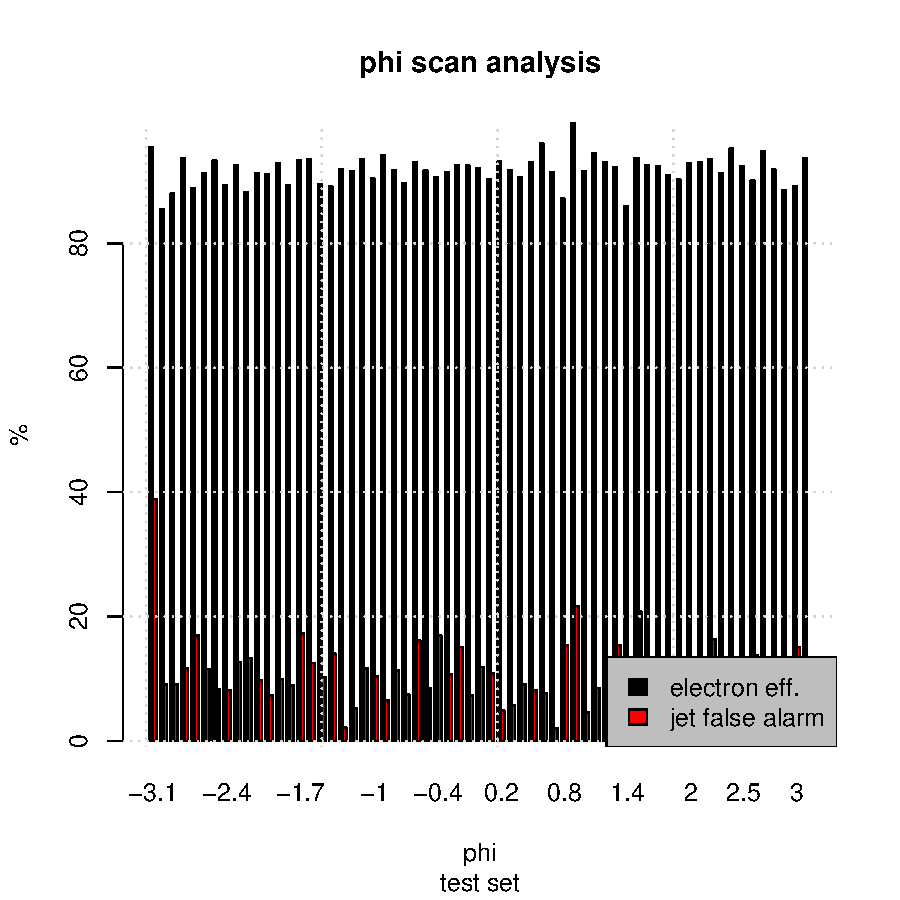
\includegraphics[scale=0.98]{eghypo/eghypo-phi-scan-test}
\end{center}
\caption{Eficiência de deteção contra falso-alarme por $\phi$ para o conjunto
de testes utilizando o algoritmo EGammaHypo.} 
\label{fig:eghypo-phi-scan-test}
\end{figure}

\begin{figure}
\begin{center}
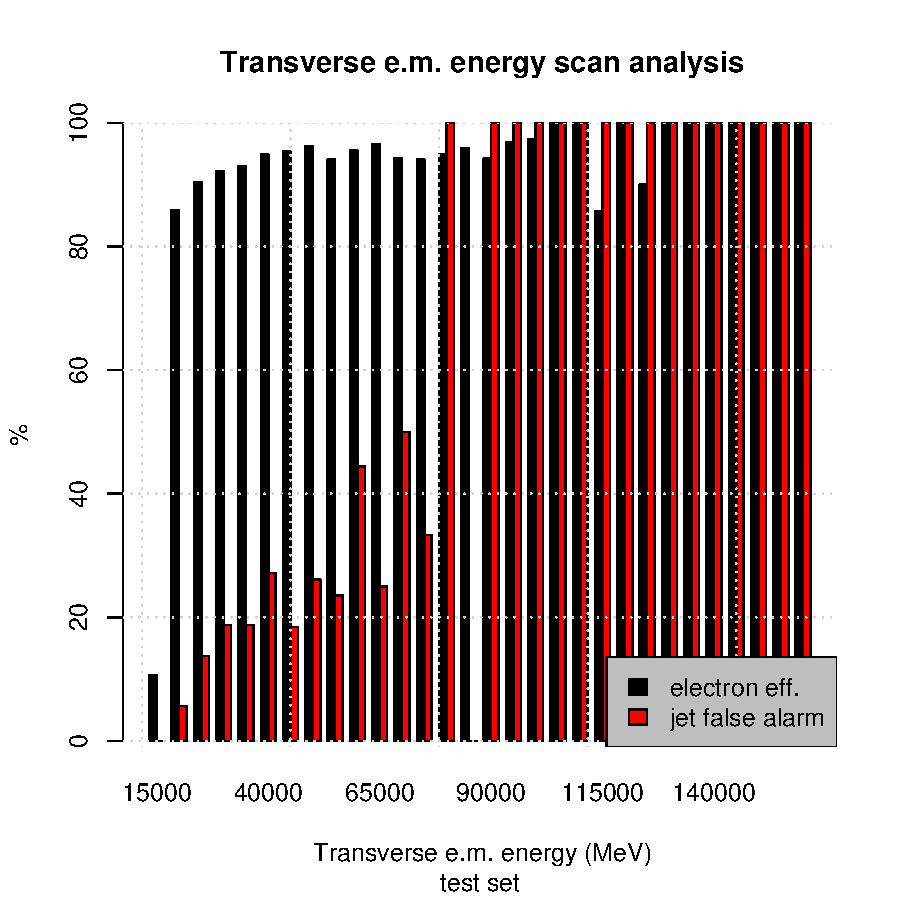
\includegraphics[scale=0.98]{eghypo/eghypo-emet-scan-test}
\end{center}
\caption{Eficiência de deteção contra falso-alarme por \etem para o conjunto
de testes utilizando o algoritmo EGammaHypo.}
\label{fig:eghypo-emet-scan-test}
\end{figure}

%\subsection{Análise de Componentes Principais}

%Isto não é óbvio que melhorará a análise do método já que temos poucas
%variáveis a a informação contida nelas traz bastante informação, mas não
%informação discriminante.

%Levando-se em consideração os dados da Tabela~\ref{tab:eghypo-partials}, é
%possível intuir que exista uma grande correlação entre as 4 variáveis
%definidas pelo T2Calo e utilizados pelo EGammaHypo para a deteção de
%elétrons. A técnica de Análise de Componentes Principais \cite{vantrees}
%define uma transformação linear que, quando aplicada a massa de dados de onde
%é originalmente extraída, completamente a descorrelaciona. Esta transformada
%é comumente conhecida como KLT (do inglês \eng{Karhunen-Loève Transform}).

%Uma das técnicas para o cálculo da KLT utiliza a matriz de covariância C do
%conjunto de dados de analisados para calcular 

%\cite{vantrees}, é possível calcular a transformação , que
%completamente descorrelacionará os dados disponíveis. 

\typeout{ *************** End of file baseline.tex *************** }
